\section{3D Geometry}
\label{sec:3d_geometry}

\begin{frame}
    \frametitle{3D coordinates}
    \begin{figure}
        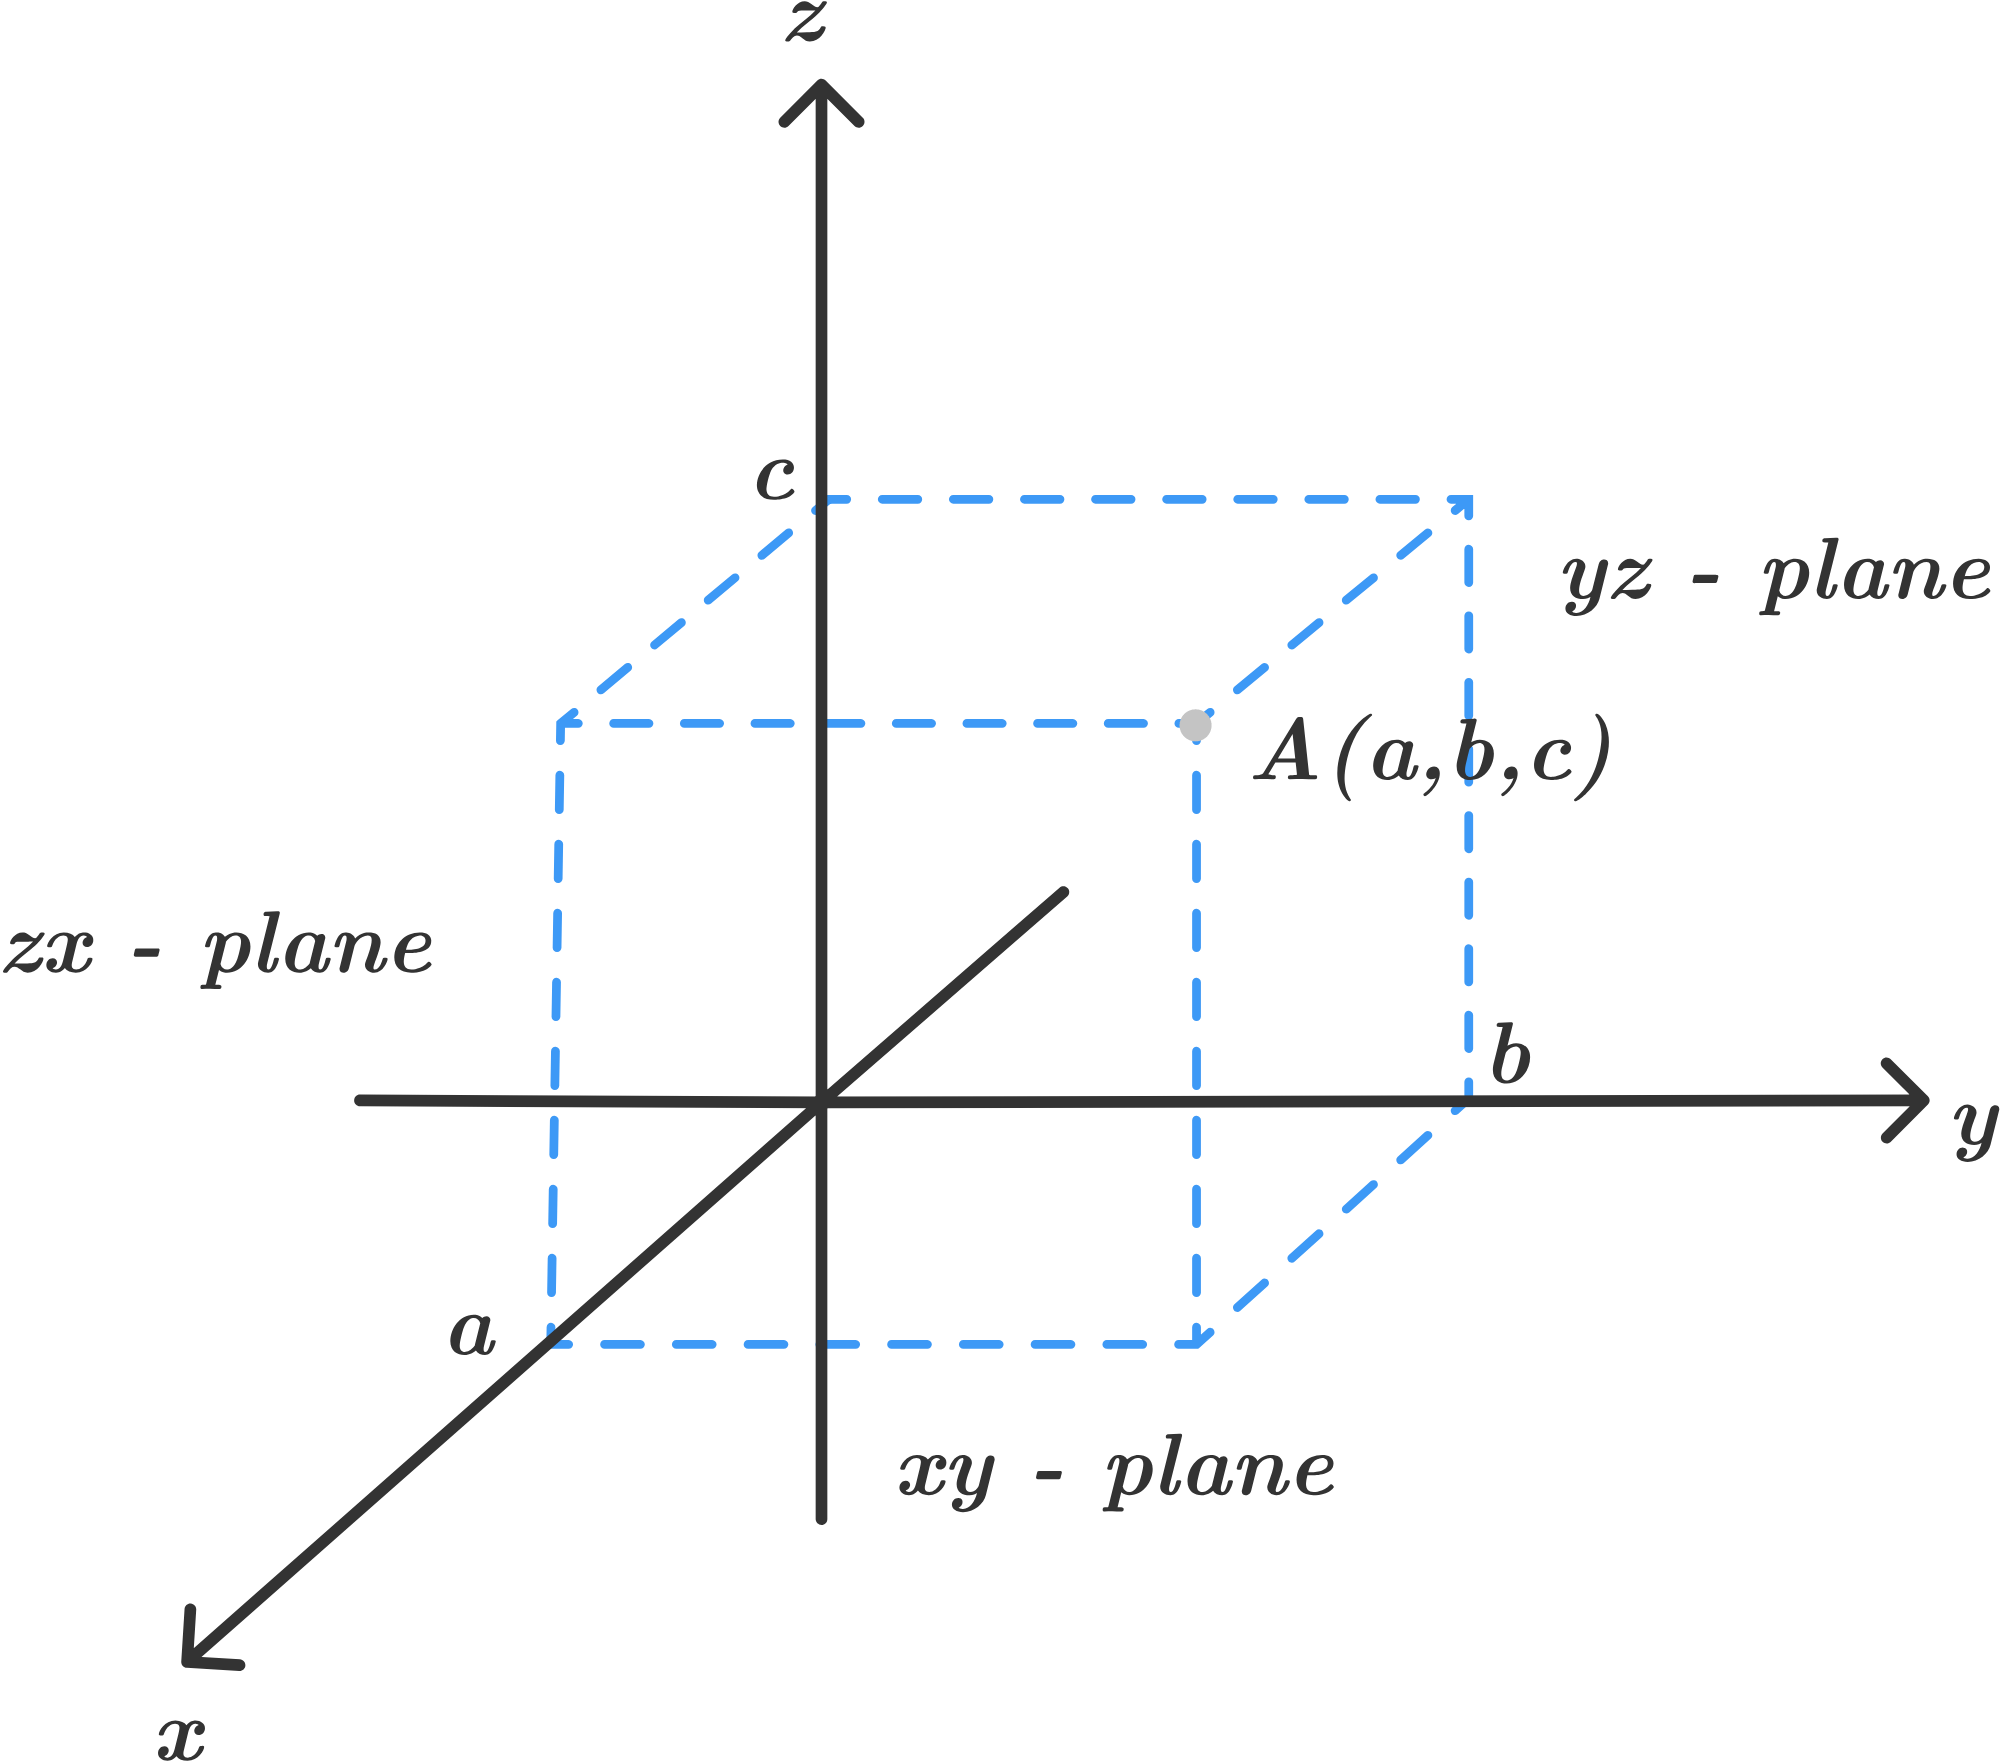
\includegraphics[scale=0.1]{3d_geometry/co_ordinate_plane.png}
        \caption{3D Coordinate Plane}
    \end{figure}
\end{frame}

\begin{frame}
    \frametitle{3D Coordinate System}
    \begin{itemize}
        \item The 3D coordinate system is defined by three mutually perpendicular axes: the x-axis, y-axis, and z-axis.
        \item A point in 3D space is represented by its coordinates \(P(x, y, z)\).
        \item The position vector of a point \(P\) in 3D space is given by:
        \[
        \vec{OP} = x\hat{\imath} + y\hat{\jmath} + z\hat{k}
        \]
    \end{itemize}       
\end{frame}

\begin{frame}
    \frametitle{Shifting the Origin}
    \begin{itemize}
        \item To shift the origin of the coordinate system, we can define a new origin point \(O'\) with coordinates \(O'(x_0, y_0, z_0)\).
        \item The position vector of a point \(P\) with respect to the new origin \(O'\) is given by:
        \[
        \vec{O'P} = (x - x_0)\hat{\imath} + (y - y_0)\hat{\jmath} + (z - z_0)\hat{k}
        \]
    \end{itemize}   
\end{frame}

